\renewcommand{\thechapter}{2}
\chapter{The EXO-200 Detector}

Among the experiments with potential to match the sensitivity of Heidelberg-Moscow is the Enriched Xenon Observatory (EXO).  In particular, the EXO-200 detector is designed to hold 200 kg of Xe enriched to 80\% in $^{136}$Xe, and anticipates probing down to $\left< m_{\beta\beta} \right> \sim 0.1$ eV~\cite{CarterICHEP}.  Xenon is a convenient material to study because it is a noble element, making it easy to purify chemically.  It has no long-lived radioactive isotopes, so there is no concern of cosmogenic activation of the Xenon while aboveground.  It has a fairly high Q-value of 2.458 MeV, giving it a larger phase-space for its decay products and putting its peak out of reach of many common backgrounds.  Xenon also provides two means to measure energy from a decay:  under the influence of an electric field, ionization charge in pure Xenon will drift; and regardless of electric field, excited Xenon scintillates.  The ratio of scintillation to ionization depends on electric field and the density of the energy deposit; thus, at high enough electric field discrimination is possible between high-energy-density $\alpha$-decay and lower-energy-density $\beta$- and $\gamma$-decay.  Another benefit of Xenon is that, since it can act as an energy detector in its pure gaseous or liquid state, it is easy to make a large monolithic Xenon detector.  We will here review how the EXO-200 experiment has been constructed to exploit these properties and explore down to interesting neutrino masses.

\begin{figure}
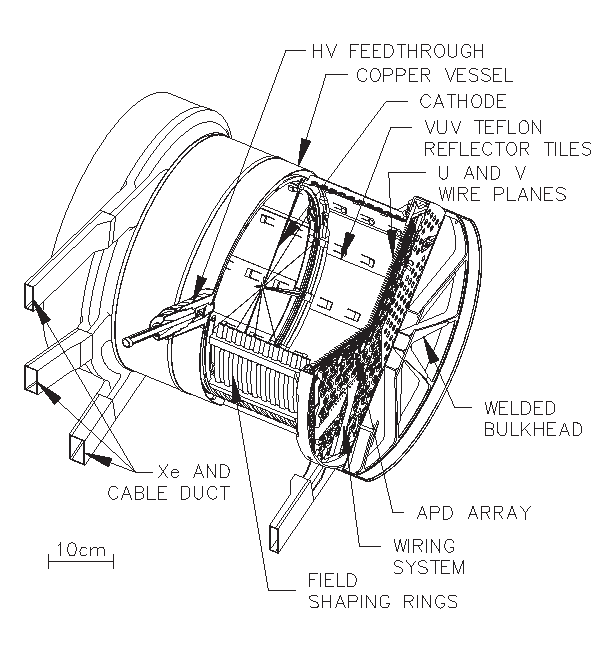
\includegraphics[scale=0.85]{TPCSchematic.eps}
\caption{Schematic of the inner EXO-200 TPC.}
\label{fig:TPCSchematic}
\end{figure}

The core of the EXO-200 detector is a cylindrical time-projection chamber (TPC), depicted in Figure~\ref{fig:TPCSchematic}, under a potential of roughly 400 V/cm.  The electric field is shaped to be parallel to the axis of the TPC throughout its fiducial volume.  The cathode is located in the middle of the TPC, and charge is collected on grids of parallel wires on either end of the TPC, giving a high-quality probe of the total ionization charge and location along one axis.  Also on both ends of the TPC, in front of these collection wires is another grid of parallel wires, orthogonal to the collection wires, which identifies an induced signal from passing ionization charge to give another position coordinate.  Finally, on both endcaps of the TPC are many large-area avalanche photodiodes (LAAPDs) which can detect the scintillation light from the primary decay~\cite{EXOLAAPD}.  The time difference between scintillation and charge collection gives a third position coordinate from a decay, and the scintillation also can give a secondary measurement of the energy of the deposit.  As noted above, comparing the scintillation and collected ionization allows $\alpha$-decays to be identified, removing one broad source of backgrounds.

The Xenon must be kept extremely pure, both to reduce backgrounds and to permit the ionization charges to drift farther with less attenuation.  To accomplish this, the detector has two pipes feeding into it so that Xenon may be circulated out of the detector continuously for repurification.  This is done using SAES Zirconium getters, which filter out all chemically reactive elements and return only noble elements.  Radioactive isotopes which are not filtered out are $^{85}$Kr (which has a Q-value much lower than that of $^{136}$Xe, making it fairly harmless) and all forms of Radon (some of whose daughter products can deposit energy around the Q-value of $^{136}$Xe).

The TPC itself is made of oxygen-free high-thermal-conductivity (OFHC) copper that was kept under concrete shielding during its time aboveground to protect it from neutron-induced activation.  Nevertheless, the copper may be a significant source of backgrounds in the energy range of interest, primarily due to natural contamination by $^{40}$K, $^{238}$U and $^{232}$Th~\cite{MaterialsCatalog}.  To mitigate this, significant effort has been expended in making the copper walls as thin as possible, averaging $1.5$ mm thick.  The ductility of copper makes such thin walls technically challenging, and a significant infrastructure has been developed to maintain the pressure of ultrapure HFE coolant, in which the TPC is immersed, so that the pressure difference can be controlled to $\sim 10$ torr.

Other significant sources of background may be the charge collection wires that pass through the TPC and the LAAPDs on its ends.  Both backgrounds have been minimized by limiting the total mass and carefully selecting materials to use.  The charge collection wires are photo-etched from phosphor bronze; the etching process was found to contribute to surface contamination, which was minimized by the use of clean etching agents and the use of a more aggressive cleaning procedure after etching~\cite{MaterialsCatalog}.  The LAAPDs are designed to minimize the radioactive contamination they introduce.  They were designed without standard ceramic encapsulation; instead the LXe is itself relied upon to insulate them.  Additionally, Aluminum used in the LAAPDs was found to be high-background, and was replaced with an acceptable substitute.  These efforts have reduced the activity introduced by the LAAPDs~\cite{MaterialsCatalog}\cite{EXOLAAPD}.

These are a few of the critical subsystems that were screened prior to use.  More details will be presented in a forthcoming detector paper to be written by the EXO collaboration.
